%----------------------------------------------------------------------------------------
%	PACKAGES AND OTHER DOCUMENT CONFIGURATIONS
%----------------------------------------------------------------------------------------

\documentclass[twoside,twocolumn,a4paper]{article}

\usepackage{blindtext} % Package to generate dummy text throughout this template 

\usepackage[T1]{fontenc} % Use 8-bit encoding that has 256 glyphs

\usepackage{lmodern}

\usepackage[hyphenbreaks]{breakurl}

\usepackage[hyphens]{url}

%\usepackage[super,sort&compress]{natbib}
%\usepackage{natbib}
%\setlength{\bibsep}{0.0pt}

\usepackage{float} %Latex toma a las figuras como "floats" esto quiere decir que se ponen donde se les canta el orto, este paquete impide que las figuras hagan lo que quieran.
\usepackage{graphicx} %figuras
\usepackage{amsmath} %me deja usar ecuaciones como la gente
\usepackage{gensymb}
\usepackage{titlesec} %PERMITE CAMBIAR EL FUCKING TAMAÑO DE LOS TITULOS Y SUBTITULOS DESPUES DE 2HS DE BUSQUEDA DE COMO MIERDA HACERLO
\titleformat{\subsection}
{\normalfont\small\bfseries}{\thesubsection}{1em}{}


\linespread{1.05} % Line spacing - Palatino needs more space between lines
\usepackage{microtype} % Slightly tweak font spacing for aesthetics

\usepackage[spanish]{babel} % Language hyphenation and typographical rules

\usepackage[numbib,notlof,notlot,nottoc]{tocbibind} % Shows bibliography as a section

\usepackage[hmarginratio=1:1,top=32mm,columnsep=20pt]{geometry} % Document margins

\usepackage[small,labelfont=bf,up,textfont=up]{caption} % Custom captions under/above floats in tables or figures

\usepackage{booktabs} % Horizontal rules in tables

\usepackage{enumitem} % Customized lists

\setlist[itemize]{noitemsep} % Make itemize lists more compact

\usepackage{abstract} % Allows abstract customization

\renewcommand{\abstractnamefont}{\normalfont\bfseries} % Set the "Abstract" text to bold

\usepackage{fancyhdr} % Headers and footers
\pagestyle{fancy} % All pages have headers and footers
\fancyhead{} % Blank out the default header
\fancyfoot{} % Blank out the default footer
\fancyhead[C]{Laboratorio 3 $\bullet$ Informe 2 $\bullet$ Grupo 8: Inafuku, Petino, Poggi} % Custom header text
\fancyfoot[C]{\thepage} % Custom footer text

\usepackage{titling} % Customizing the title section

\usepackage{hyperref} % For hyperlinks in the PDF

%----------------------------------------------------------------------------------------
%	TITLE SECTION
%----------------------------------------------------------------------------------------

\setlength{\droptitle}{-4\baselineskip} % Move the title up

\pretitle{\begin{center}\LARGE\bfseries} % Article title formatting
\posttitle{\end{center}} % Article title closing formatting
\title{Caracterizaci\'on de diodos. Rectificadores de media y onda completa.} % Article title
\author{%
\textsc{Maximiliano Inafuku} \\[1ex] % Your name
\normalsize \href{mailto:maxi-46@hotmail.com}{maxi-46@hotmail.com} % Your email address
\and % Uncomment if 2 authors are required, duplicate these 4 lines if more
\textsc{Ernesto Petino} \\[1ex] % Second author's name
\normalsize \href{mailto:ernesto.atmo@gmail.com}{ernesto.atmo@gmail.com} % Second author's email address
\and % Uncomment if 2 authors are required, duplicate these 4 lines if more
\textsc{Ignacio Poggi} \\[1ex] % Second author's name
\normalsize \href{mailto:ignaciop.3@gmail.com}{ignaciop.3@gmail.com} % Second author's email address
}

\date{Grupo 8 - Laboratorio 3, C\'atedra Bilbao - Departamento de F\'isica, Facultad de Ciencias Exactas y Naturales, Universidad de Buenos Aires \newline \\ \today} % Leave empty to omit a date
\renewcommand{\maketitlehookd}{%
\begin{abstract}
\noindent En este trabajo se estudi\'o la utilizaci\'on del diodo semiconductor como elemento de rectificaci\'on de corriente alterna, en combinaci\'on con otros elementos (resistencias y capacitores). Como primera experiencia, se construy\'o un rectificador de media onda conformado por un circuito simple conformado por una fuente alterna, una resistencia y un diodo semiconductor en serie; en segundo lugar se conform\'o un rectificador de onda completa utilizando un puente de diodos semiconductores en paralelo a una resistencia recorrida en un solo sentido por la corriente, y mediante el agregado de un condensador en paralelo a esta resistencia, la aproximaci\'on a corriente continua y observaci\'on del ripple.
\end{abstract}
}

%----------------------------------------------------------------------------------------

\begin{document}

% Print the title
\maketitle


%----------------------------------------------------------------------------------------
%	ARTICLE CONTENTS
%----------------------------------------------------------------------------------------

\section{Introducci\'on}

El diodo es un dispositivo de dos terminales que permite el paso de la corriente en una sola direcci\'on. Los m\'as utilizados actualmente son los diodos semiconductores y Zener (Figura \ref{fig:tipos_diodos}).\par

Cuando se somete al diodo semiconductor a una diferencia de tensi\'on externa, puede polarizarse de forma directa o inversa. En la polarizaci\'on directa, la bater\'ia disminuye la barrera de potencial, permitiendo el paso de la corriente de electrones a trav\'es de la uni\'on; es decir, el diodo polarizado directamente funciona como un conductor, cuando se supera un cierto voltaje umbral. En el caso de la polarizaci\'on inversa, el polo negativo de la bater\'ia se conecta a la zona p y el polo positivo a la zona n, lo que hace aumentar la zona de carga, y la tensi\'on en dicha zona hasta que se alcanza el valor de la tensi\'on de la bater\'ia. \par

Otro tipo de diodo estudiado es el diodo Zener. Estos se emplean para producir una tensi\'on entre sus terminales muy constante y relativamente independiente de la corriente que los atraviesan. Normalmente, polarizados en forma inversa no permite pr\'acticamente el pasaje de corriente, pero al alcanzar una determinada tensi\'on (tensi\'on Zener), se produce un aumento de la cantidad de corriente que lo atraviesa, manteniendo la tensi\'on entre sus terminales pr\'acticamente constante. 

\begin{figure}[h]
\captionsetup{justification=centering}
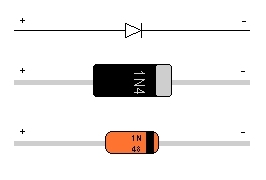
\includegraphics[width=\linewidth]{tipos_diodos.jpg}
\caption{Clases de diodos estudiados. De arriba hacia abajo: diagrama de un diodo, diodo semiconductor y diodo Zener.}
\label{fig:tipos_diodos}
\end{figure}

El modelo utilizado para caracterizar al diodo es el de Shockley, el cual permite aproximar el comportamiento del mismo en la mayor\'ia de los circuitos. La ecuaci\'on que relaciona la intensidad de corriente y la diferencia de potencial es \cite{eq:shockley}:
\begin{equation}
\label{eq:shockley}
I = I_{S}(e^\frac{V_{D}}{nV_{T}} - 1)
\end{equation}

donde

\begin{itemize}
\item 
$V_{D}$: Tension a trav\'es del diodo. 
\item 
$I_{S}$: Intensidad de corriente de saturaci\'on que se establece al polarizar inversamente el diodo ($\sim 10^{-12}$ A).
\item
$V_{T}$: Tension t\'ermica ($\sim$ 25 mV a 25$\degree$C). Se define como $\frac{kT}{q}$, donde $k$ es la constante de Boltzmann, $T$ la temperatura y $q$ la carga del electr\'on.
\item
$n$: Factor de calidad.
\end{itemize}

La ecuaci\'on (\ref{eq:shockley}) da lugar a una curva caracter\'istica (Figura \ref{fig:curva_shockley}) con los siguientes par\'ametros:

\begin{itemize}
\item 
$V_{u}$: Tensi\'on umbral. Al polarizar directamente el diodo, la barrera de potencial inicial se va reduciendo, incrementando la corriente ligeramente. Sin embargo, cuando la tensi\'on externa supera la tensi\'on umbral, la barrera de potencial desaparece.
\item 
$I_{max}$: Intensidad de corriente m\'axima que puede conducir el diodo sin fundirse.
\item
$V_{r}$: Tensi\'on de ruptura. A partir de un determinado valor de la tensi\'on, el diodo comienza a conducir tambi\'en en polarizaci\'on inversa. 
\end{itemize}

\begin{figure}[h]
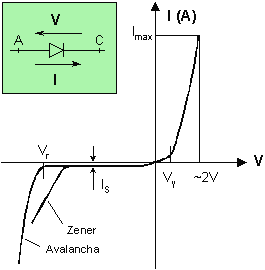
\includegraphics[width=\linewidth]{curva_shockley.jpg}
\captionsetup{justification=centering}
\caption{Curva caracter\'istica de un diodo seg\'un el modelo de Shockley.}
\label{fig:curva_shockley}
\end{figure}


\textbf{Rectificadores de media onda y onda completa.} \newline
\par
Los rectificadores el\'ectricos son los circuitos encargados de convertir la corriente alterna en corriente continua. Los m\'as habituales son los construidos con diodos. Los dos tipos de rectificadores estudiados en este trabajo son los rectificadores de media onda y los rectificadores de onda completa. \par

Los rectificadores de media onda funcionan haciendo pasar la mitad de la corriente alterna a trav\'es de uno o m\'as diodos, convirtiendo en este paso dicha mitad de la corriente alterna en corriente el\'ectrica directa. Estos rectificadores no son muy eficientes porque s\'olo convierten la mitad de la corriente alterna en corriente directa; por lo tanto, solo un diodo es necesario para su funcionamiento.\par

Los rectificadores de onda completa son m\'as complejos que los rectificadores de media onda, pero tambi\'en son mucho m\'as eficientes. Estos generalmente utilizan cuatro diodos para funcionar (puente de diodos), haciendo pasar la corriente alterna a trav\'es de dicho puente, obteniendo un terminal positivo y otro negativo, caracter\'istico de la corriente directa.


%------------------------------------------------

\section{Dispositivo experimental}
Los instrumentos de laboratorio utilizados fueron:
\begin{itemize}
\item 
\label{diodo} Diodos Schottky (1N 4007 LD). % Estos son los diodos normales
\item 
\label{zener} Diodo Zener.
\item 
\label{osc} Osciloscopio Tektronix 1052-B (R\'otulo: OSC-067). %el rotulo lo chamuye de otro experimento que hicimos porque no lo tenia, si alguien lo anoto, mejor
\item
\label{trans} Transformador conectado a l\'inea. 
\item Resistencias varias.
\item Capacitores varios.
\end{itemize}

Para poder caracterizar el voltaje umbral del diodo, es necesario conocer la ca\'ida de potencial y la intensidad que pasan por el mismo. Con el objetivo de hallar estos datos se arm\'o el circuito que se muestra en la Figura \ref{fig:dsp_exp}, donde se utiliz\'o como volt\'imetro al osciloscopio y la fuente alterna, es el transformador conectado a l\'inea. Esta configuraci\'on fue la misma tanto para la caracterizaci\'on del Schottky como la del diodo Zener. Los datos se recogieron en la computadora conectando el osciloscopio a la misma por medio de un cable USB, utilizando el programa OpenChoice Desktop. \par 

\begin{figure}[H]
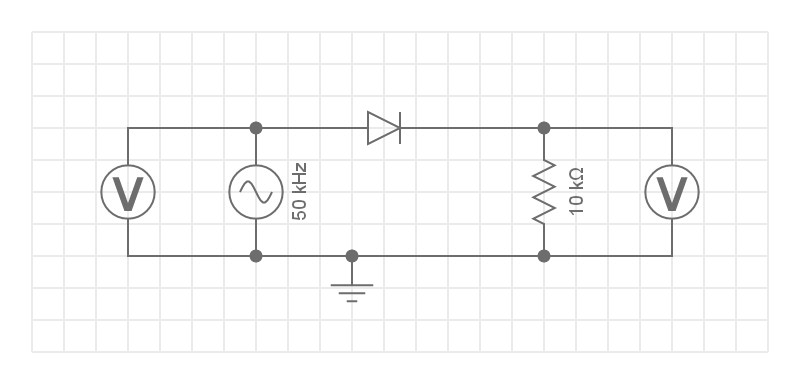
\includegraphics[width=\linewidth]{disp_exp.png}
\captionsetup{justification=centering}
\caption{Esquema del circuito realizado para la caracterizaci\'on del diodo.}
\label{fig:dsp_exp}
\end{figure}

Para la segunda parte de la experiencia, se arm\'o un puente de diodos como el que se muestra en la Figura \ref{fig:disp_exp2}. Esta vez, la parte del circuito de inter\'es fue c\'omo era el voltaje que pasaba por la resistencia de carga, por lo que se coloc\'o all\'i el osciloscopio y se observ\'o el voltaje en funci\'o del tiempo. Luego para una \'ultima experiencia se modific\'o levemente el circuito anterior, agregando un capacitor en paralelo a la resistencia de carga (Figura \ref{fig:disp_exp3}).Se observ\'o para este caso que ocurr\'ia con la ca\'ida de potencial al utilizar distintos capacitores. \par 

\begin{figure}[h]
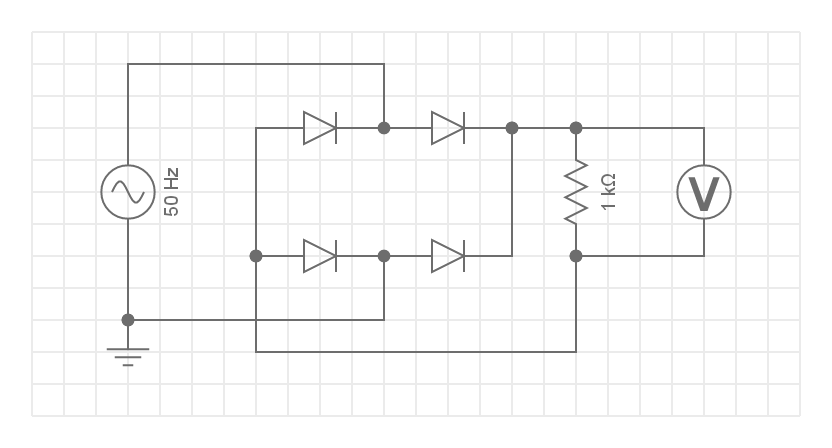
\includegraphics[width=\linewidth]{disp_exp2.png}
\captionsetup{justification=centering}
\caption{Esquema del circuito realizado del rectificador de onda completa.}
\label{fig:disp_exp2}
\end{figure}

Para poder apreciar mejor la forma funcional del Ripple, se utiliz\'o la opci\'on del osciloscopio "DC coupling", la cu\'al remueve la parte continua de la se\~nal y permite ver la oscilaci\'on centrada en el cero. 

\begin{figure}[H]
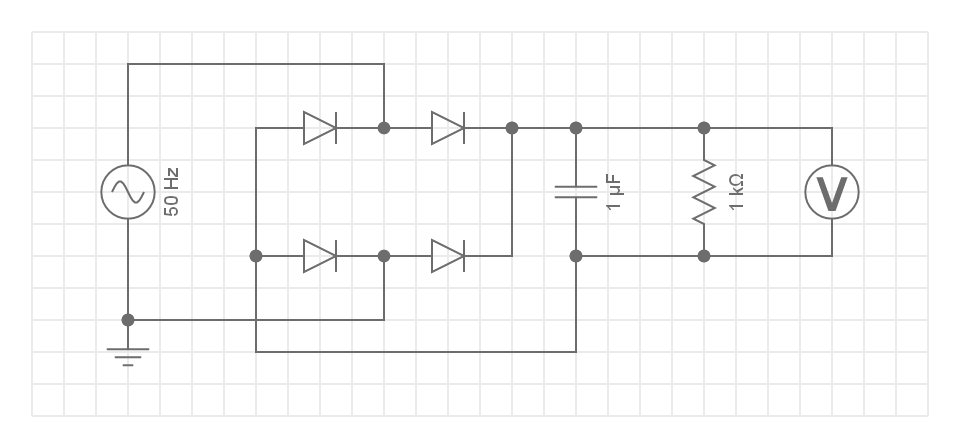
\includegraphics[width=\linewidth]{disp_exp3.png}
\captionsetup{justification=centering}
\caption{Esquema del circuito realizado, agregando un capacitor al rectificador de onda completa.}
\label{fig:disp_exp3}
\end{figure}

%------------------------------------------------
%------------------------------------------------

\section{Resultados y an\'alisis}

\subsection{Caracterizaci\'on de diodos Schottky y Zener}

Lo primero que se puede apreciar en el osciloscopio es que la ca\'ida de potencial de la resistencia es nula cu\'ando la fuente de alterna tiene un potencial negativo, indicando que la corriente circulando por la resistencia era nula. Y cuando el voltaje entregado por la fuente es positivo, si se logra observar una diferencia de potencial no nula en la resistencia (Figura ~\ref{fig:diodo2}). Por este motivo el nombre de esta configuraci\'on es rectificador de media onda, ya que "permite el paso de media onda". Adem\'as es posible notar que la frecuencia registrada del osciloscopio se encuetra en un valor cercano a los 50 Hz, que es la frecuencia de la tensi\'on de l\'inea, como se esperaba.

\begin{figure}[h]
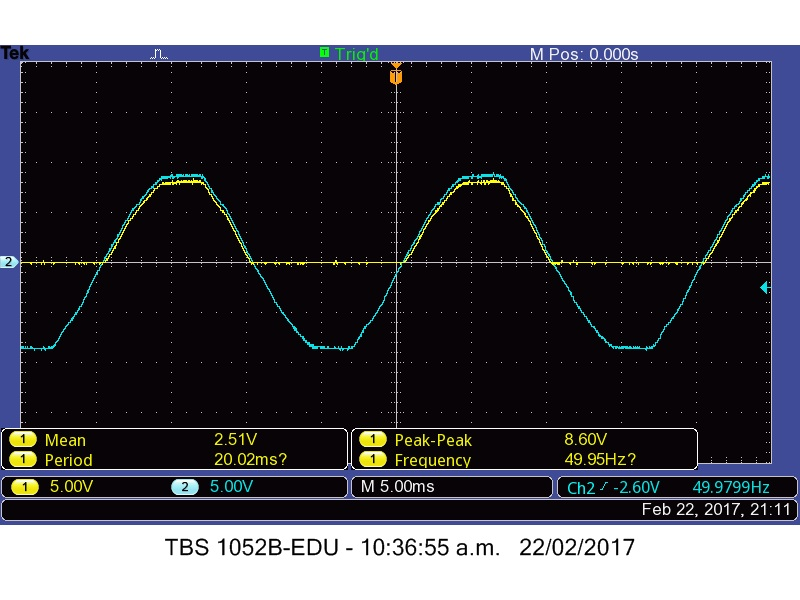
\includegraphics[width=\linewidth]{Diodo.jpg}
\captionsetup{justification=centering}
\caption{Captura de pantalla obtenida por el osciloscopio, con el diodo Schottky. En amarillo la ca\'ida de potencial de la resistencia y en azul el voltaje entregado por la fuente alterna.}
\label{fig:diodo2}
\end{figure}

Con los datos de la ca\'ida de potencial en la resistencia y el voltaje otorgado por el transformador conectado a la red de l\'inea se obtuvieron la intensidad que circulaba por el diodo y la ca\'ida de potencial del mismo por medio de las ecuaciones:

\begin{gather}
I=\frac{V_R}{R} \\
V_D=V-VR
\end{gather}

Siendo la resistencia utilizada en este circuito de unos 10 k$\Omega$.
\bigbreak

Al graficar la intensidad en funci\'on de la ca\'ida de potencial en el diodo, se puede observar que a voltajes negativos (polarizaci\'on inversa respecto al diodo) la intensidad es pr\'acticamente nula, mientras que luego de pasar una cierta tensi\'on umbral, $V_u$, el diodo se comporta casi como un conductor, aumentando la corriente que pasa por este de forma considerable (Figura ~\ref{fig:diodo_shock}). Se hice hizo un ligero cambio respecto al modelo de Shockley original, que fue denominar a $nV_T = V_{Teff}$ ya que al realizar el ajuste, estos dos par\'ametros son indistinguibles.

\begin{figure}[h!]
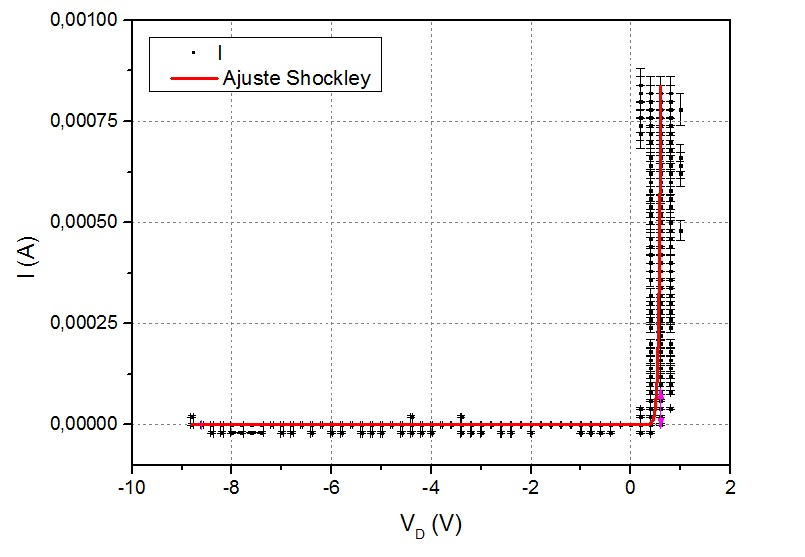
\includegraphics[width=\linewidth]{diodograph.jpg}
\captionsetup{justification=centering}
\caption{Gr\'afico de la intensidad circulante por el diodo en funci\'on de su ca\'ida de potencial.}
\label{fig:diodo_shock}
\end{figure}

La determinaci\'on de dicho $V_u$ es arbitraria, pero se suele tomar como criterio, el voltaje al cu\'al la intensidad es de 1 mA. Ajustando la curva obtenida con el modelo de Shockley los par\'ametros obtenidos se muestran en la Tabla ~\ref{tab:diodo}. Se estima entonces, con los par\'ametros obtenidos del modelo que $V_u\approx0.6V$. Cabe destacar que esta es s\'olo una estimaci\'on ya que el alto error en el par\'ametro $I_S$ no permiti\'o obtener este valor con exactitud. El $R^2$ no es muy favorable, con lo que muchos datos no son explicados correctamente por el modelo, pero el alto valor obtenido del F-valor indica que es improbable que el ajuste haya sido aleatorio. El modelo utilizado tuvo una gran complicaci\'on para ajustar los datos, debido a que este era muy sensible a los valores del $V_D$ en cu\'anto comenzaba el crecimiento exponencial. \par 

\begin{table}[h!]
\centering
\captionsetup{justification=centering}
%\setlength{\belowcaptionskip}{-10pt} Esto saca el espacio debajo de las caption
\caption{Ajuste de Shockley}
\label{tab:diodo}
\begin{tabular}{|c|c|}
\hline
\multicolumn{2}{|c|}{$I(V_D)=I_S . (e^\frac{V_D}{V_{Tee}}-1)$} \\ \hline
$I_S$                       & $5*10^{-11}\pm2*10^{-9}$                   \\ \hline
$V_{Teff}$                  & $0.040\pm0.006$                  \\ \hline
$R^2$                       & 0.5                              \\ \hline
F-valor                     & 2700                             \\ \hline
\end{tabular}
\end{table}

En el gr\'afico de los residuos se puede ver que estos est\'an discretizados debido a la digitalizaci\'on del instrumental utilizado. En general se observa que para valores bajos, las desviaciones son negativas, y se llega a observar que en los \'ultimos valores, donde se observa el comportamiento exponencial del ajuste, los residuos aumentan (Figura ~\ref{fig:res}).

\begin{figure}[H]
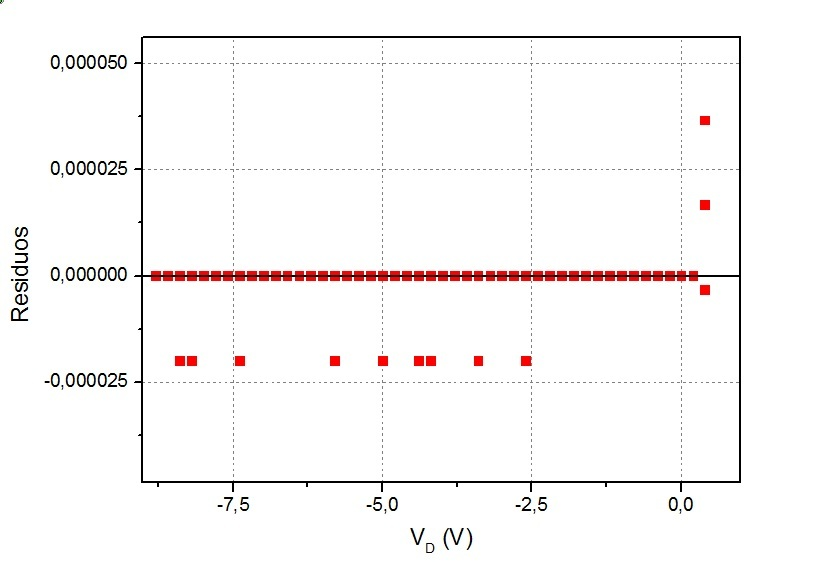
\includegraphics[width=\linewidth]{residuos.jpg}
\captionsetup{justification=centering}
\caption{Gr\'afico de los residuos obtenidos por el ajuste con el model de Schottky.}
\label{fig:res}
\end{figure} 

El otro diodo estudiado fue el llamado diodo Zener, cuyas caracter\'isticas en polarizaci\'on directa son an\'alogas a las del diodo Schottky, pero que en polarizaci\'on inversa se comporta de manera distinta ($V <$ 0).


Cuando el diodo esta polarizado inversamente, una peque\~na corriente circula por \'el, llamada corriente de saturaci\'on $I_{S}$, esta corriente permanece relativamente constante mientras se aumenta la tensi\'on inversa hasta que el valor de \'esta alcanza $V_{Z}$, llamada tensi\'on Zener ($V_{Z} = - 0.8$ V en este caso), para la cual el diodo entra en la regi\'on de colapso, donde la corriente empieza a incrementarse r\'apidamente.

Se observ\'o que en esta regi\'on, peque\~nos cambios de tensi\'on produc\'ian grandes cambios de corriente. Al realizar el ajuste, se vi\'o que el modelo de Shockley ajustaba correctamente la zona donde el diodo se encuentra polarizado directamente; pero no donde el diodo Zener muestra su comportamiento particular, por lo tanto se busc\'o una leve modificaci\'on a dicho modelo para tratar de aproximar dicha zona:

\begin{equation}
\label{eq:shockley2}
I = \left\{ \begin{array}{lcc}
             I_{S}(e^\frac{V_{D}}{nV_{T}} - 1) &   si  & V_{D} \geq 0 \\
             \\ I_{S}(-e^\frac{-V_{D} - V_{Z}}{nV_{T}} + e^\frac{V_{D}}{nV_{T}} - 1) &  si  & V_{D} \leq 0
             \end{array}
   \right.
\end{equation}

Nuevamente, se obtuvieron la intensidad que circulaba por el diodo y la ca\'ida de potencial del mismo por medio de las ecuaciones (2) y (3), solo que en este circuito la resistencia utilizada fue de 680 $\Omega$.

\begin{figure}[h]
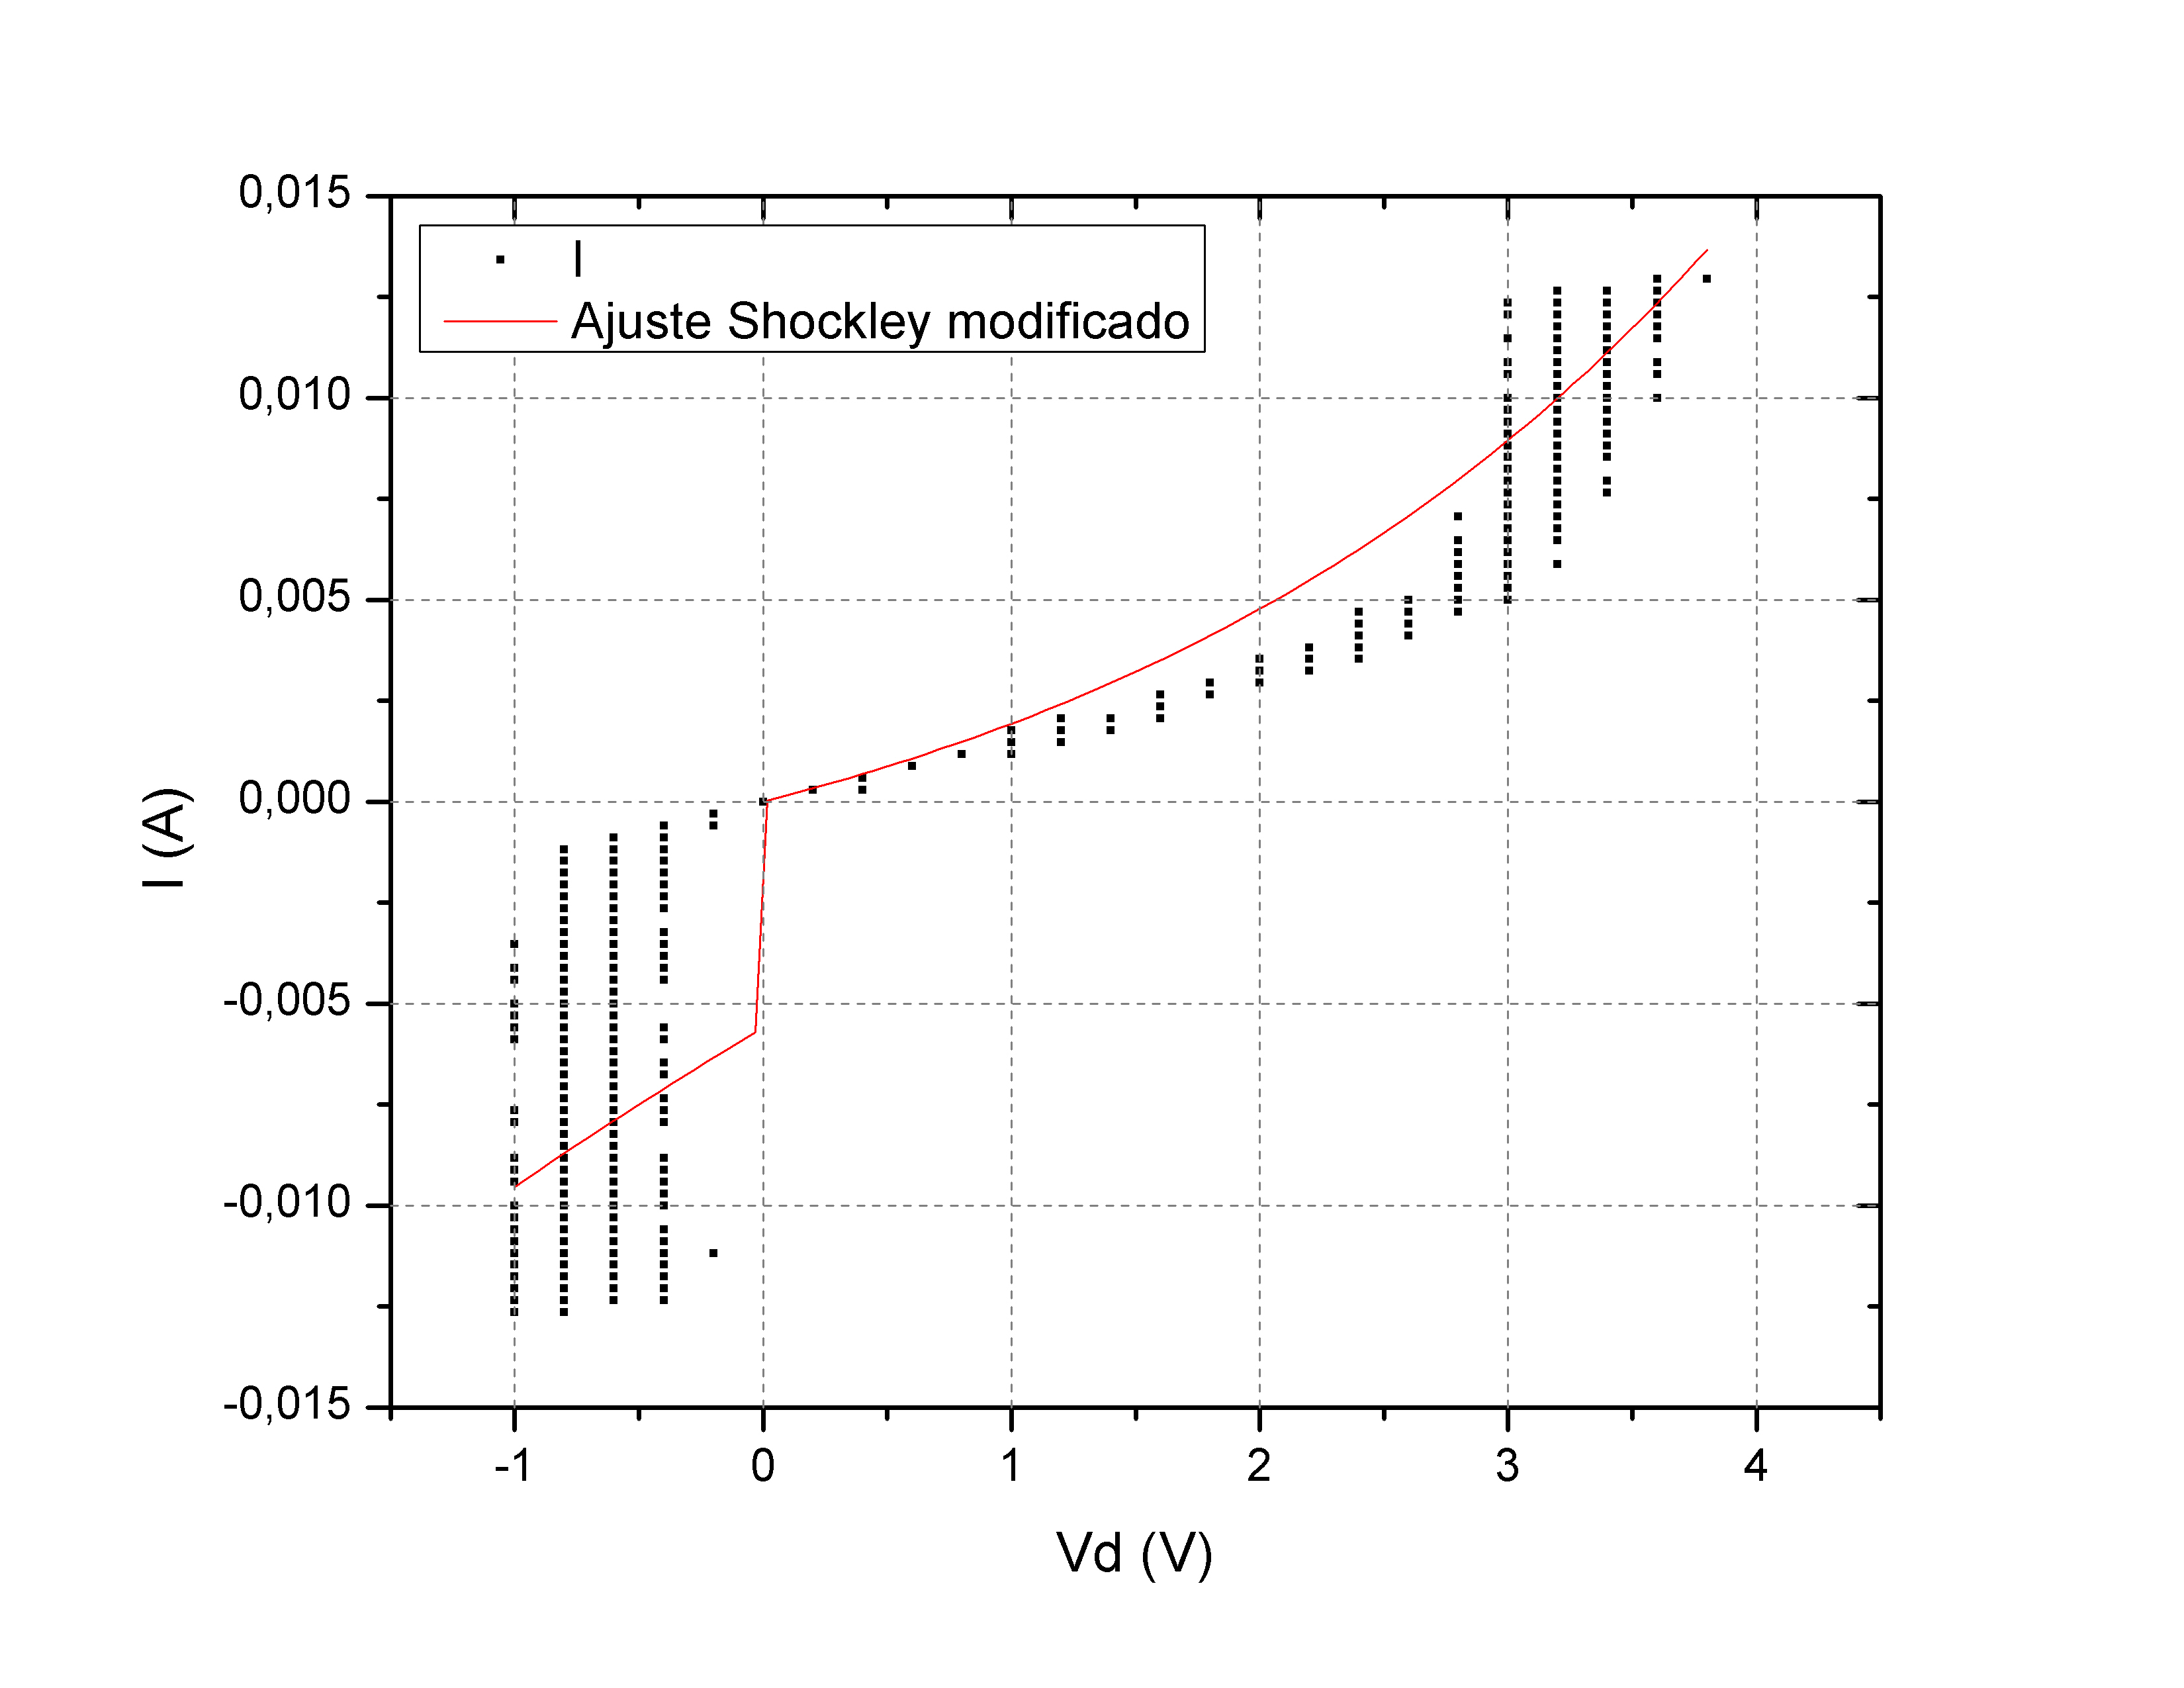
\includegraphics[width=\linewidth]{zener_ajuste.jpg}
\captionsetup{justification=centering}
\caption{Gr\'afico de la intensidad circulante por el diodo Zener funci\'on de su ca\'ida de potencial.}
\label{fig:zener_ajuste}
\end{figure} 

Ajustando la curva obtenida con el modelo de Shockley modificado (los par\'ametros obtenidos se muestran en la Tabla ~\ref{tab:zener}), se observa que a medida que se va aumentando negativamente el voltaje aplicado al diodo, la corriente que pasa por \'el aumenta muy poco ($\sim$ 1,2 mA), pero una vez que se llega a un determinado voltaje, llamada voltaje o tensi\'on de Zener ($V_{Z}$), el aumento del voltaje (siempre negativamente) es muy peque\~no, pudiendo considerarse constante, como puede verse en la Figura ~\ref{fig:zener_ajuste} para los valores de $V < 0$.\par
En este caso, el valor de $R^2$ mejoro mucho con respecto al diodo Schottky, con lo cual gran parte de los datos son explicados correctamente por el modelo, ademas de que la cifra obtenida del F-valor indica que es improbable que el ajuste haya sido aleatorio. 
En este caso tambi\'en cabe destacar que el modelo utilizado tuvo una gran complicaci\'on para ajustar los datos, debido a que este era muy sensible a los valores de $V_{D}$ y $V_{Z}$ en cuanto comenzaba el crecimiento exponencial.

\begin{table}[h!]
\centering
\captionsetup{justification=centering}
%\setlength{\belowcaptionskip}{-10pt} Esto saca el espacio debajo de las caption
\caption{Ajuste de Shockley modificado para el diodo Zener. Nuevamente, $nV_{T} = V_{Teff}$.}
\label{tab:zener}
\begin{tabular}{|c|c|}
\hline
\multicolumn{2}{|c|}{$I(V_D)$ = Ecuaci\'on ~\ref{eq:shockley2}} \\ \hline
$I_S$                       & $411*10^{-5}\pm6,53*10^{-5}$                   \\ \hline
$V_{Teff}$                  & $2.594\pm0.030$                  \\ \hline
$R^2$                       & 0.905                              \\ \hline
F-valor                     & 11871                            \\ \hline
\end{tabular}
\end{table}

En el gr\'afico de los residuos se observa que para valores entre $V_{u}$ y $V_{Z}$, las desviaciones son negativas, y se llega a observar que en los valores en los extremos, tanto para los valores negativos y positivos de V, donde se observa el comportamiento exponencial del ajuste, los residuos aumentan (Figura ~\ref{fig:zener_residuos}).

\begin{figure}[H]
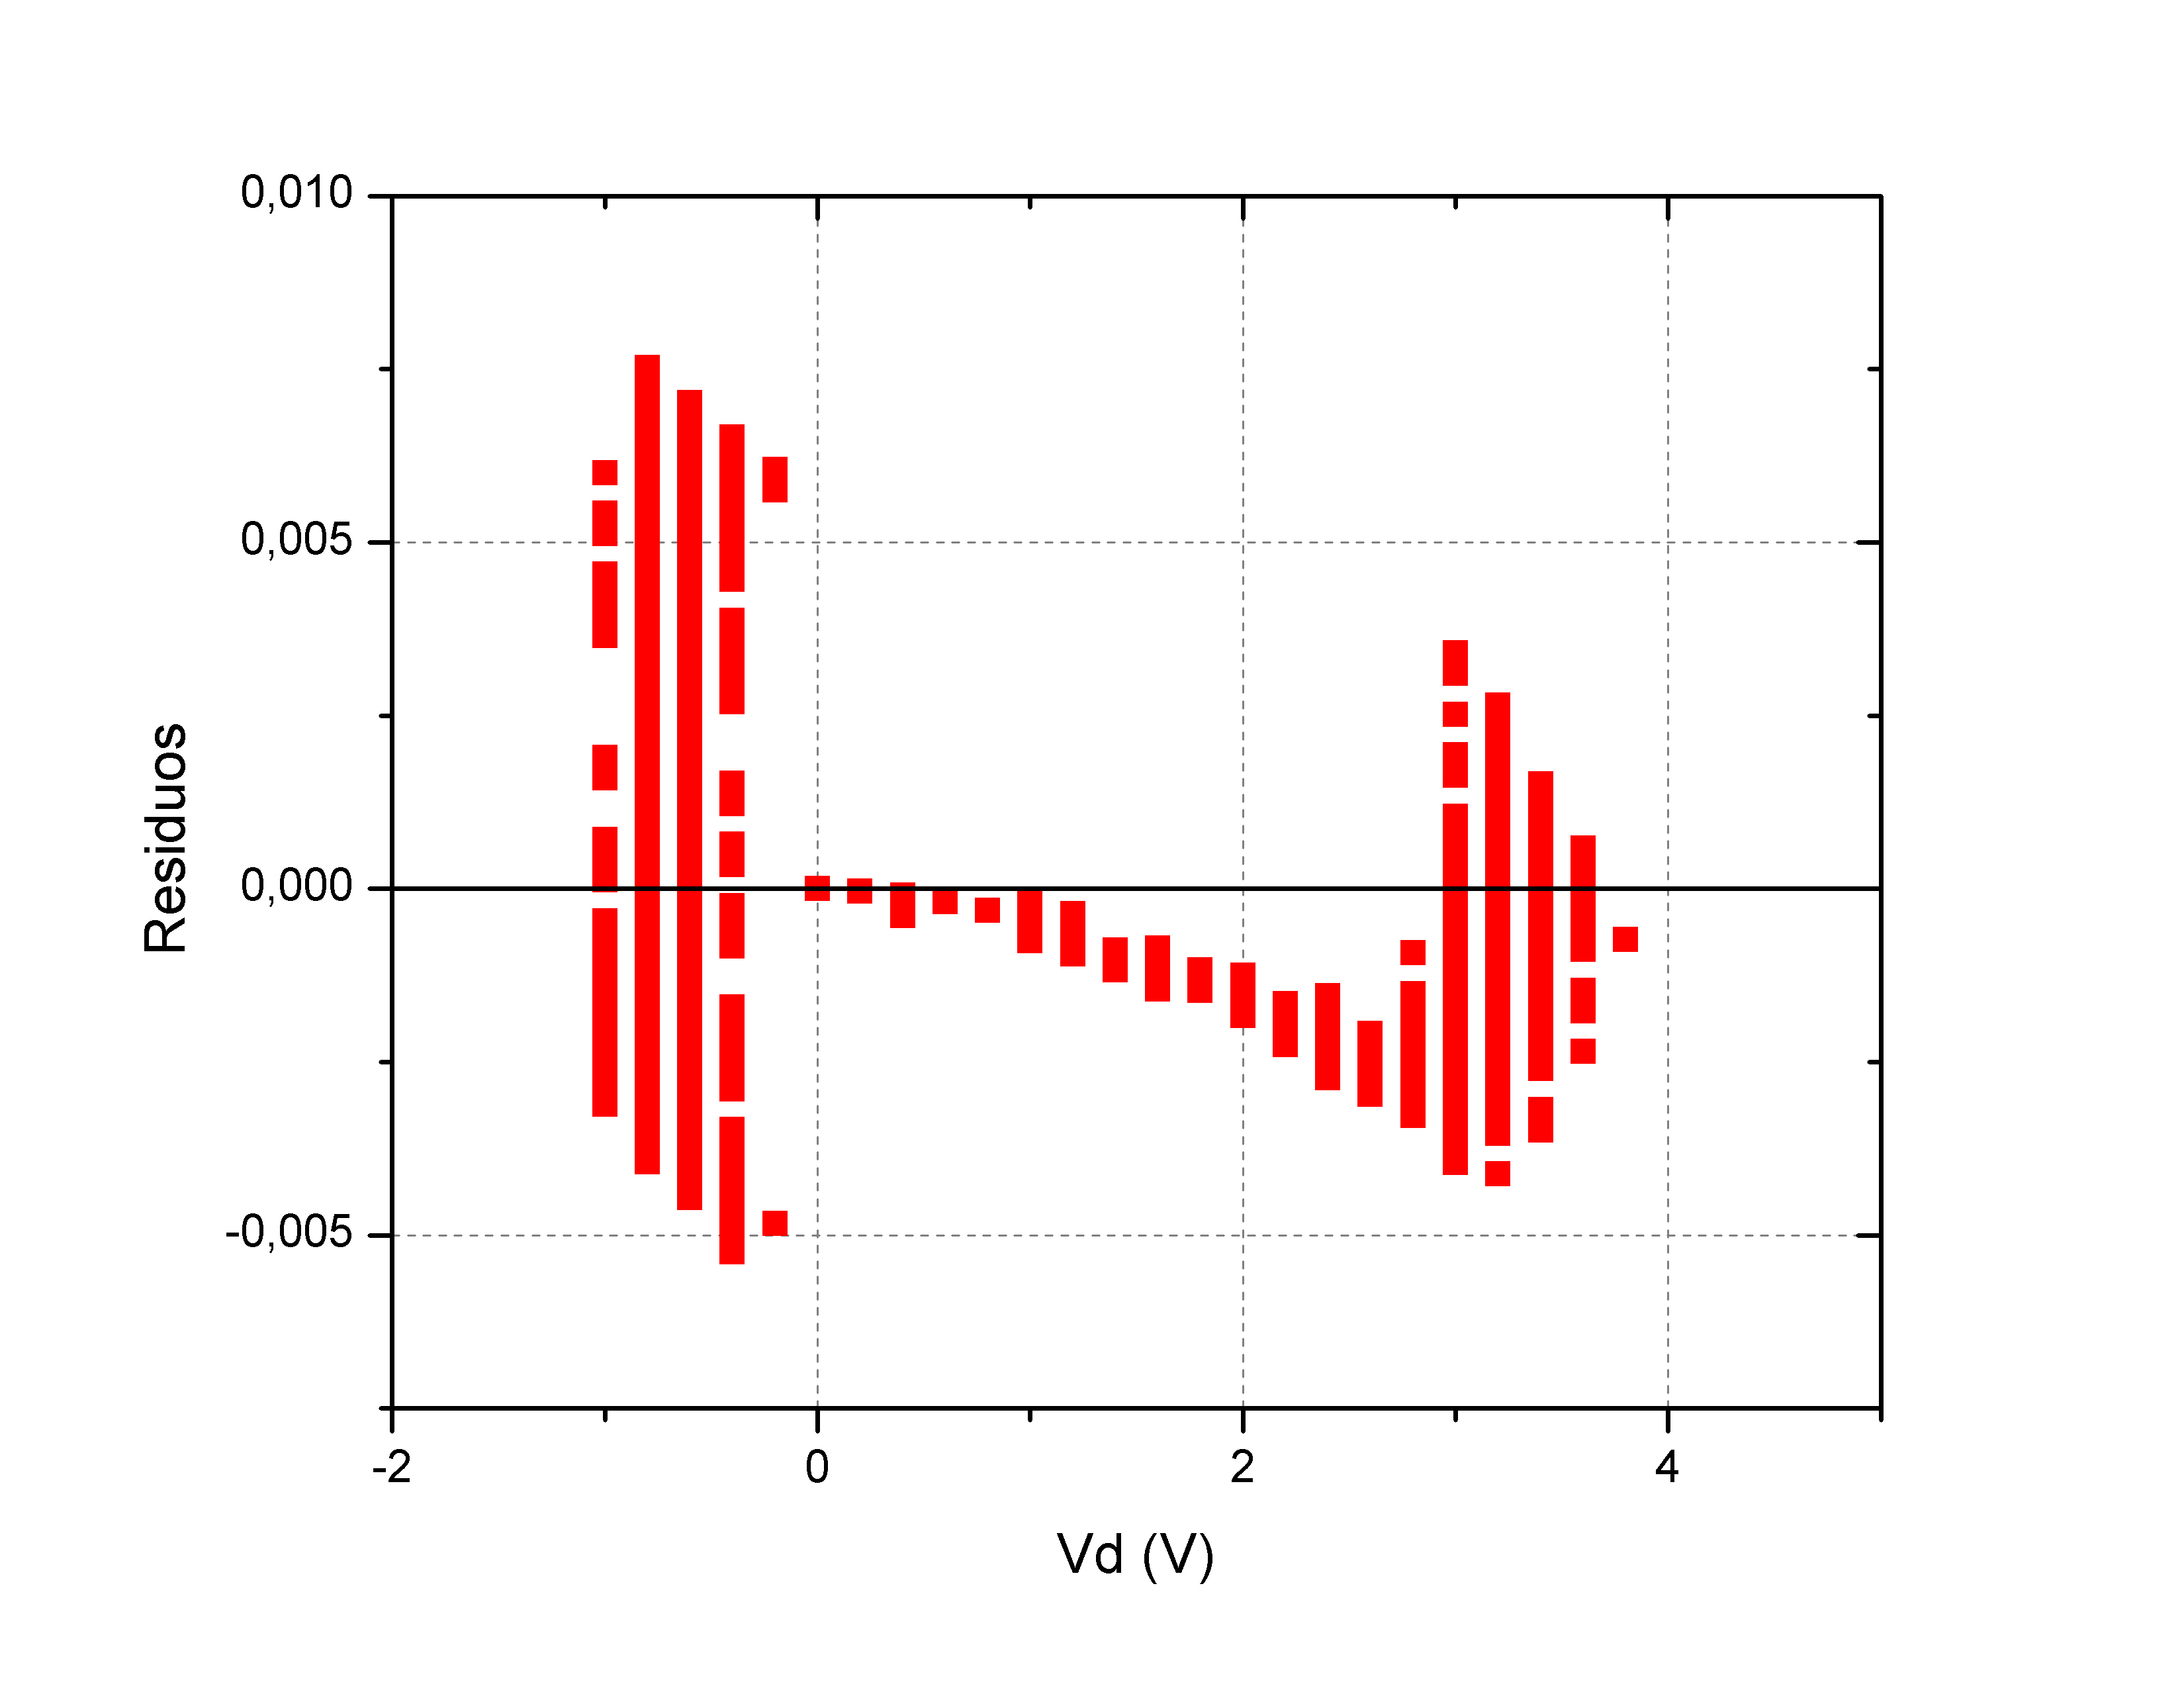
\includegraphics[width=\linewidth]{zener_residuos.jpg}
\captionsetup{justification=centering}
\caption{Gr\'afico de los residuos obtenidos por el ajuste con el modelo de Shockley modificado para el diodo Zener.}
\label{fig:zener_residuos}
\end{figure}

%------------------------------------------------
\subsection{Rectificadores de onda completa y observaci\'on del Ripple}
En esta segunda parte del experimento se realiz\'o un an\'alisis m\'as bien cualitativo de un rectificador de onda completa y del fen\'omeno del Ripple. Se arm\'o entonces el puente de diodos (Figura \ref{fig:disp_exp2}) y se observ\'o en el osciloscopio como variaba la ca\'ida de potencial en funci\'on del tiempo (Figura \ref{fig:noripple}).\par

\begin{figure}[h]
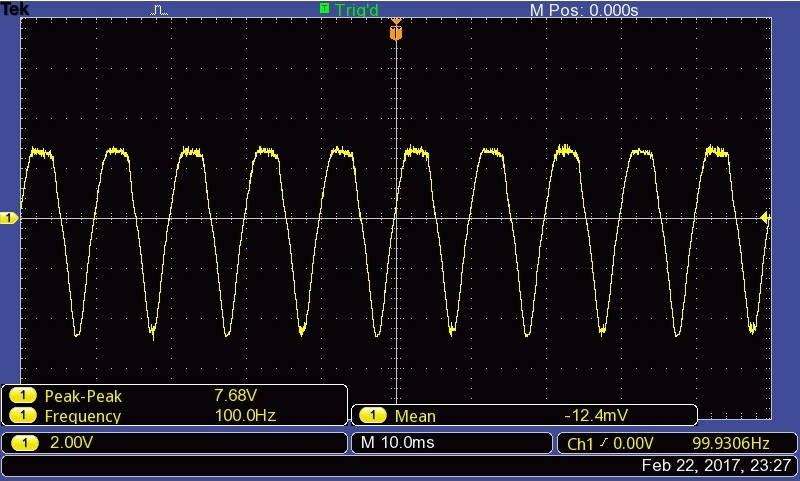
\includegraphics[width=\linewidth]{noripple.jpg}
\captionsetup{justification=centering}
\caption{Rectificador de onda completa}
\label{fig:noripple}
\end{figure} 

En este caso el voltaje oscila, siendo siempre positivo, y la apariencia es similar al m\'odulo de una sinusoidal. El voltaje pico a pico entregado por la fuente de corriente alterna es de $17.4\pm0.2$ V, mientras que la ca\'ida de potencial de la resistencia es de unos $7.68\pm0.06$ V. Este es menor a $8,7\pm0.1$ V (la mitad de lo entregado por la fuente), por lo que hay una leve atenuaci\'on de la corriente circuito. Por otro lado la frecuencia observada es de aproximadamente 100 Hz, que es justamente el doble a los 50 Hz entregados por la fuente de corriente alterna como se esperaba. Al invertir la corriente cu\'ando la ca\'ida de potencial es negativa, justamente se obtiene una funci\'on cuyo per\'iodo es el doble del voltaje sinusoidal entregado por la fuente.\par 


Al agregar un capacitor de en paralelo a la resistencia de carga, sobre la cu\'al se mide la ca\'ida de potencial, se produce el efecto de "ripple". El primer capacitor agregado es de 226 nF, en este caso el efecto observado es bastante tenue, siendo ahora la oscilaci\'on de $6.24\pm0.06$ V. En cambio al colocar un capacitor de 4.24 $\mu$F, la oscilaci\'on se vi\'o fuertemente disminu\'ida, siendo de tan solo $1.28\pm0.06$ V. Por \'ultimo con un capacitor de 62 $\mu$F, la oscilaci\'on se hace casi imperceptible por el osciloscopio y esta se distorsiona considerablemente, siendo la oscilaci\'on de aproximadamente 218 mV. La Figura \ref{fig:ripplejunto} muestra una imagen compuesta por todos los ripples observados y el caso del circuito sin ning\'un capacitor. Todas las im\'agenes preservan la escala temporal (10 ms por cada rect\'angulo) y s\'olo la \'ultima modifica la escala de voltaje (cambiando de 2 V a 50 mV por cada rect\'angulo).

\begin{figure}[h]
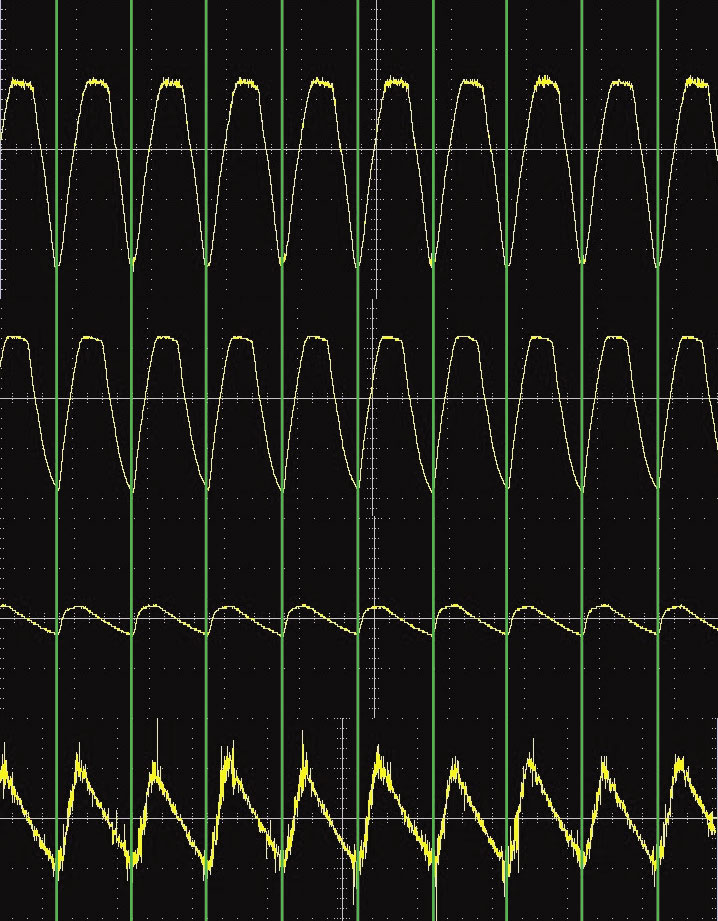
\includegraphics[width=\linewidth]{ripplejunto.jpg}
\captionsetup{justification=centering}
\caption{Comparaci\'on del efecto ripple seg\'un la capacidad colocada. De arriba hacia abajo, sin ning\'un capacitor, con un capacitor de 226 nF, uno de 4.24 $\mu$F y por \'ultimo uno de 62 $\mu$F.}
\label{fig:ripplejunto}
\end{figure} 

Cabe destacar que al agregar mayor capacidad, m\'as se reducen las oscilaciones del rectificador de onda completa original. Sin embargo, la frecuencia de las oscilaciones se mantiene igual, como se muestra en la Figura \ref{fig:ripplejunto}, dado por el hecho de que todos los m\'inimos coinciden. 

%------------------------------------------------
%------------------------------------------------


\section{Conclusiones}


%----------------------------------------------------------------------------------------
%	REFERENCE LIST
%----------------------------------------------------------------------------------------

\begin{thebibliography}{99} % Bibliography - this is intentionally simple in this template

\bibitem{intro} Robert L. Nashelsky ,Boylestad Louis. 2009. Electr\'onica: Teor\'ia de circuitos y dispositivos electr\'onicos. M\'exico: Pearson educaci\'on.  
\bibitem{osc} Tektronix. Marzo del 2012. TBS1000B and TBS1000B-EDU Series, Digital Storage Oscilloscopes, User Manual. [accedido el 26 de Febrero del 2017] \url{http://www.phys.uconn.edu/~eyler/phys3150/R/TBS1052B_User_Manual.pdf}
\bibitem{eq:schokley2} J. Mike Rollins. Enero del 2008. Zener Diode Simulator. [accedido el 26 de Febrero del 2017]. \url{http://www.camotruck.net/rollins/simulator.html}
 
\end{thebibliography}

%----------------------------------------------------------------------------------------

\end{document}
